\section{Implementation}
\label{sec:impl}

As discussed in Section~\ref{sec:bg}, the cost of AIMer is concentrated in binary-field arithmetic repeated across all parties and in a large number of Keccak calls. This section reduces these costs using AVX-512. The basic idea consists of two parts. The first is to place the data of multiple parties side by side in a 512-bit register and process them simultaneously with a single instruction. The second is to merge several bit operations into a single instruction.

The existing AVX2 implementation, which we use as the baseline, stores the element of only \emph{one party} in a 128-bit register. It then processes one party at a time using PCLMULQDQ. This limitation comes from the AVX2 PCLMULQDQ instruction, whose VEX-encoded form operates on 128-bit XMM operands. In this section, we explain how this limitation is overcome with 512-bit registers. We describe binary-field multiplication in Section~\ref{sec:field}, the linear layer in Section~\ref{sec:matmul}, and Keccak in Section~\ref{sec:keccak}.

\subsection{Binary-Field Arithmetic: Four-Party Parallel Multiplication per 512-Bit Register}
\label{sec:field}

An element of $\gftwo{128}$ is 128 bits long. Thus, it fits exactly into one 128-bit \emph{lane}. A 512-bit ZMM register can store \emph{four} such lanes. Therefore, elements from four different parties can be loaded side by side into a single register. The key instruction, VPCLMULQDQ, multiplies these four lanes independently without cross-lane interference. As a result, four $64\times64\to128$ carry-less multiplications, one for each party, are completed with a single instruction. This contrasts with AVX2, which requires four instructions to perform the same work.

When two 128-bit elements are multiplied, the result can grow up to 256 bits. However, an element of the field $\gftwo{128}$ must always be 128 bits long. Therefore, the upper part of the product is reduced back to 128 bits according to the irreducible polynomial. This modular reduction is also applied identically to the four lanes, so the four parties are processed together.

Squaring and multiply-accumulate operations are also grouped in units
of four parties. For $\gftwo{128}$, squaring is completed with two
carry-less multiplications because the intermediate cross terms vanish. In sections where several products must be added consecutively, modular reduction is not performed after every multiplication. Instead, the products are accumulated first, and reduction is performed only once at the end. Modular reduction is an expensive operation. By delaying it and applying it once, its cost can be amortized over multiple products.

Elements of $\gftwo{192}$ and $\gftwo{256}$ occupy 1.5 and 2 128-bit lanes, respectively. The 256-bit case uses exactly two lanes. Thus, four parties fit into two ZMM registers without unused space. In contrast, the 192-bit case requires 1.5 lanes. The remaining 0.5 lane is filled with zero padding. Therefore, part of the lane capacity is wasted in the 192-bit variants.

\subsection{Linear Layer: Combining Two Operations into One Instruction with VPTERNLOGQ}
\label{sec:matmul}

The linear layer multiplies an input vector by a binary matrix. The result is equal to the XOR of all rows whose corresponding input bits are 1. Therefore, the implementation scans the input bits one by one. If a bit is 1, the corresponding row is XORed into the accumulator. If a bit is 0, the row is skipped.

The issue is the conditional branch implied by ``if the bit is 1.'' Branching is inefficient in SIMD code. Therefore, we replace the branch with \emph{masking}. The branch-free procedure is as follows. First, one input bit is expanded into a value filled with the same bit. If the bit is 1, the expanded value consists entirely of 1s. If the bit is 0, it consists entirely of 0s. When this mask is ANDed with the row, the row remains unchanged if the bit is 1. If the bit is 0, the result becomes all zero. This value is then XORed into the accumulator.

\begin{algorithm}[h]
\caption{Linear-layer accumulation: mask generation and VPTERNLOGQ}
\label{alg:matmul}
\begin{algorithmic}[1]
\Require Party element $a=(h\,\|\,l)$ (upper and lower 64 bits), matrix rows $\mathrm{row}_0,\dots,\mathrm{row}_{127}$, accumulator $k$
\Statex \textit{($h,\,l,\,k,\,\mathrm{row}_j$ are 512-bit registers whose 64-bit lanes contain four parties)}
\For{$j \gets 63$ \textbf{downto} $0$} \Comment{Upper 64 bits}
\State $\mathrm{mask} \gets \Call{Asr}{h,\,63}$ \Comment{Arithmetic right shift by 63: replicate the most significant bit to the full 64-bit word ($1\!\to\!\texttt{1{\dots}1}$, $0\!\to\!\texttt{0{\dots}0}$)}
\State $k \gets \Call{Vpternlogq}{k,\ \mathrm{mask},\ \mathrm{row}_{64+j},\ \texttt{0x78}}$ \Comment{$k \oplus (\mathrm{mask}\wedge \mathrm{row})$, AND+XOR in one instruction}
\State $h \gets \Call{Shl}{h,\,1}$ \Comment{Move the next bit to the most significant position}
\EndFor
\For{$j \gets 63$ \textbf{downto} $0$} \Comment{Lower 64 bits, repeated identically with $l$ and $\mathrm{row}_{j}$}
\State $\mathrm{mask} \gets \Call{Asr}{l,\,63}$;\quad $k \gets \Call{Vpternlogq}{k, \mathrm{mask}, \mathrm{row}_{j}, \texttt{0x78}}$;\quad $l \gets \Call{Shl}{l,\,1}$
\EndFor
\State \Return $k$
\end{algorithmic}
\end{algorithm}

The key point is that the computation ``AND the mask with the row and then XOR the result into the accumulator'' is a single \emph{three-input bitwise logic} operation. In AVX2, this requires \emph{two instructions}, AND and XOR. In contrast, \textbf{VPTERNLOGQ} in AVX-512 evaluates an arbitrary three-input bitwise logic function in \emph{one instruction}.

\subsection{Keccak: AVX-512VL Acceleration}
\label{sec:keccak}

We accelerate the Keccak permutation using the same two ideas described above. In this case, we use the \textbf{AVX-512VL} extension. AVX-512VL allows AVX-512 instructions to be used with 256-bit \emph{YMM} registers.

\subsubsection{Packing Multiple Hashes into One Register}

AIMer invokes the same Keccak permutation many times. Therefore, as shown in Fig.~\ref{fig:interleaving}, we interleave four Keccak states. The same 64-bit lane from each state is placed side by side in one 256-bit YMM register, giving $4\times64=256$ bits per lane group. Then, a single instruction processes the corresponding lanes of four states at the same time. As a result, four hash computations proceed in parallel.

\begin{figure}[h]
\centering
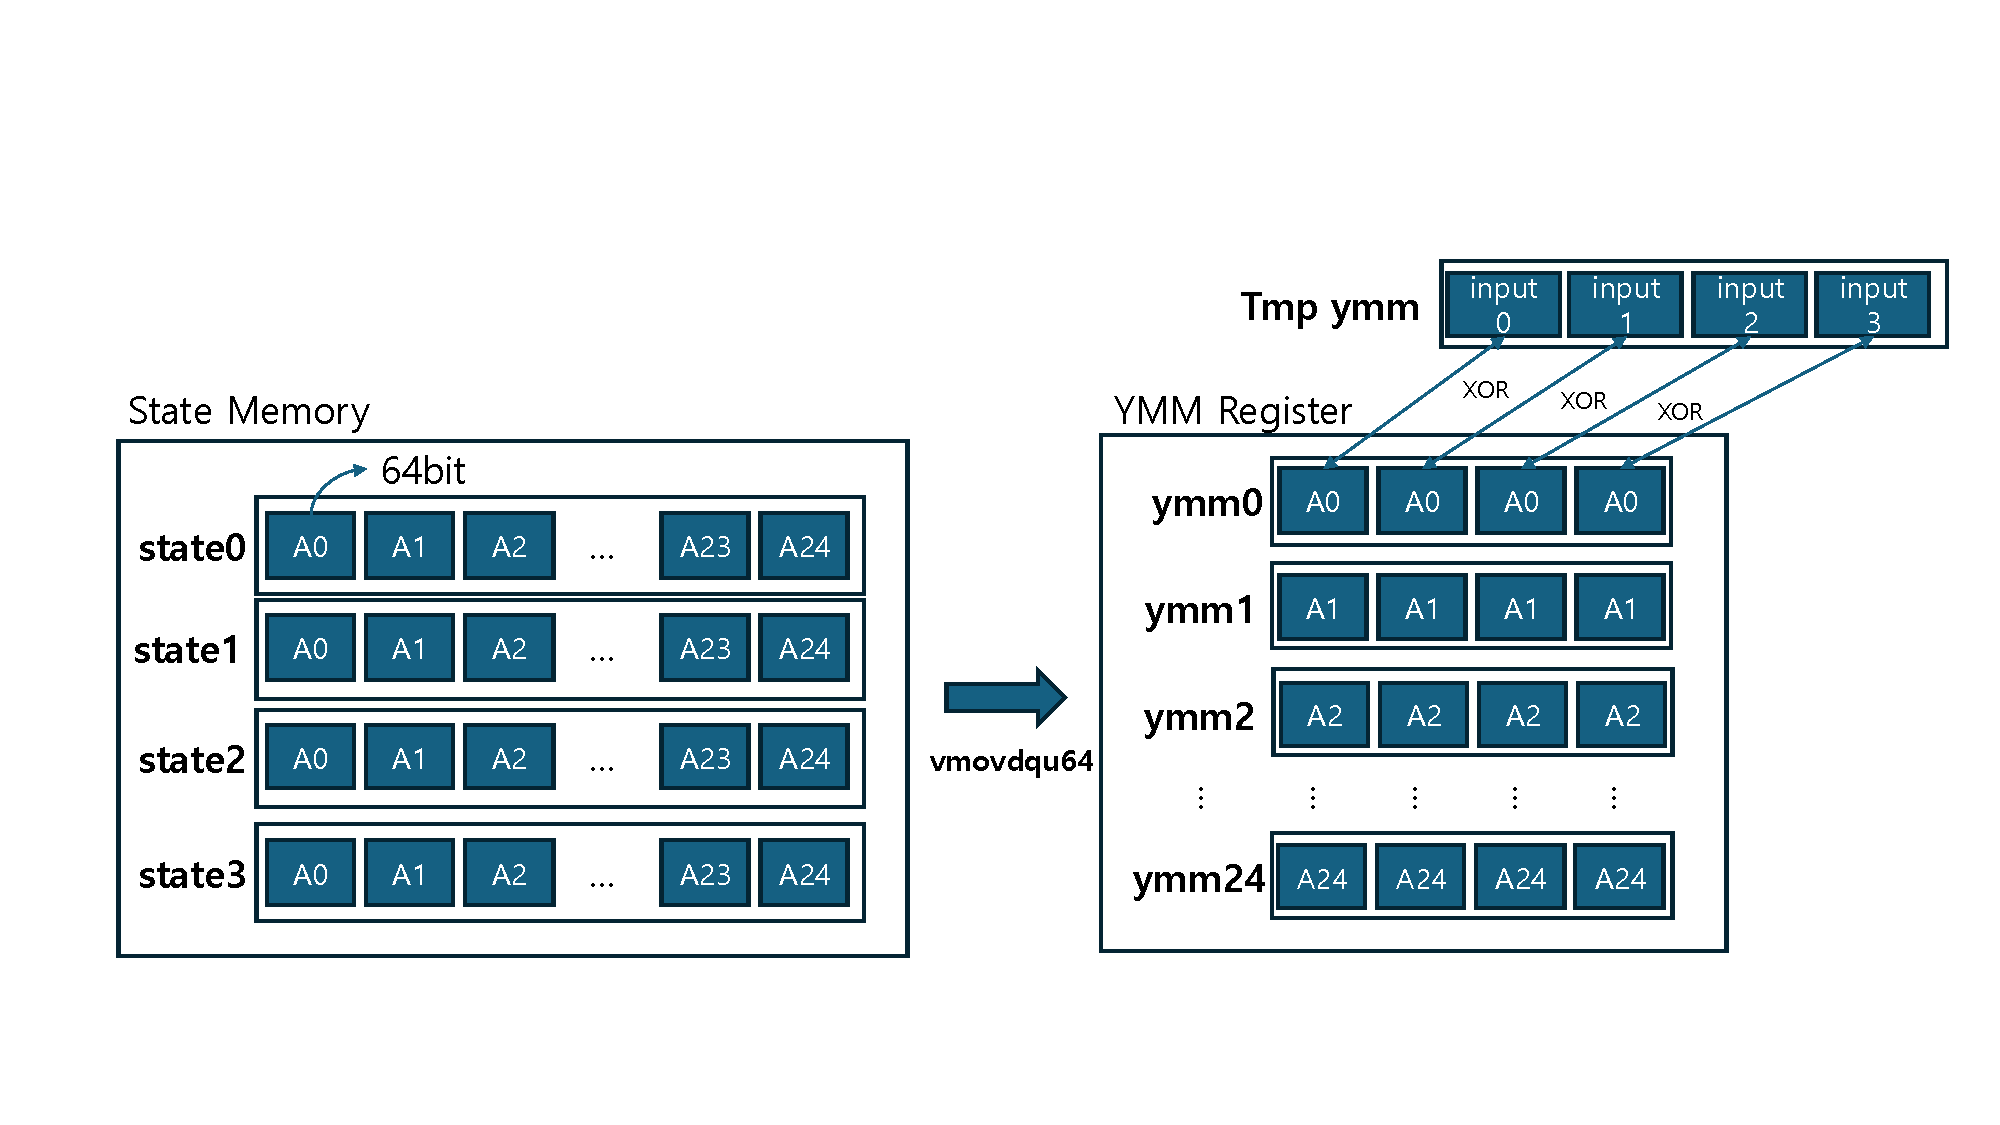
\includegraphics[width=0.9\linewidth]{figure/interleaving.pdf}
\caption{The same lanes from four Keccak states are collected into one 256-bit YMM register. The blue A0 lanes from the four states form ymm0.}
\label{fig:interleaving}
\end{figure}

\subsubsection{Merging Multiple Operations into One Instruction}

Each round of the Keccak permutation consists of five steps. Among them, the dominant operations are \emph{bit rotations} and \emph{logical operations}. The rotation step rotates each 64-bit lane by a fixed amount. AVX2 implements this with three instructions: left shift, right shift, and OR. In contrast, \texttt{vprolq} performs the same operation with a single instruction.

The three XOR operations in the diffusion step and the nonlinear operation $a\oplus(\lnot b\wedge c)$ are both \emph{bitwise logic operations over three inputs}. Therefore, each of them can be handled by one VPTERNLOGQ instruction.
